%!TEX root = ../dissertation.tex

\chapter{Results and Discussion}
\label{cha4:results}
\section{Simulator}
Baseline = [0.0 0.0 0.0537]'
\subsection{Rotation estimation error}
\subsubsection{Simulation Parameters}
\begin{itemize}
	\item Maximum Matches : $30$
	\item False Matches : $10 \%$ of maximum matches
	\item Good Matches : $50 \%$ of the maximum matches
	\item Noise $\sigma^2$ : $10 \ px$
	\item Number of saccades: $45$
	\item Zmin : $0.05 m$
	\item Zmáx : $5 m$
\end{itemize}
\subsubsection{Experiment 1 - Saccade amplitudes generated with $\sigma^2 = 4 \degree $}

\begin{minipage}{0.33\textwidth}
	\centering
	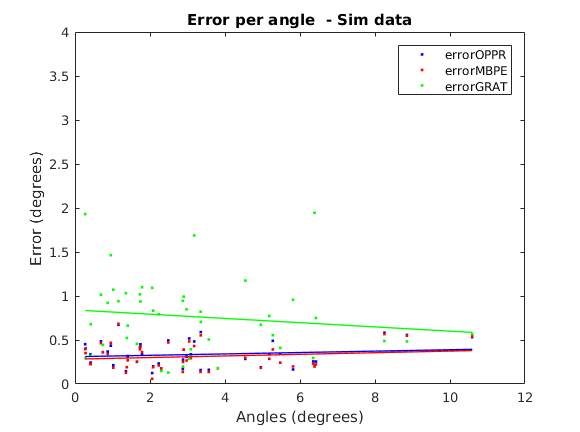
\includegraphics[width=\textwidth]{images/sim/10anglex.png}
	\captionof{figure}{Error per saccade amplitude (in degrees) under simulation on the horizontal axis.}
	\label{cha5:sec1:10anglex}
\end{minipage}
\begin{minipage}{0.33\textwidth}
	\centering
	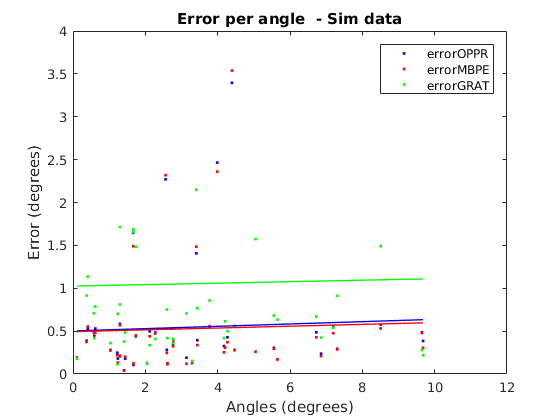
\includegraphics[width=\textwidth]{images/sim/10angley.png}
	\captionof{figure}{Error per saccade amplitude (in degrees) under simulation on the vertical axis.}
	\label{cha5:sec1:10angley}
\end{minipage}
\begin{minipage}{0.33\textwidth}
	\centering
	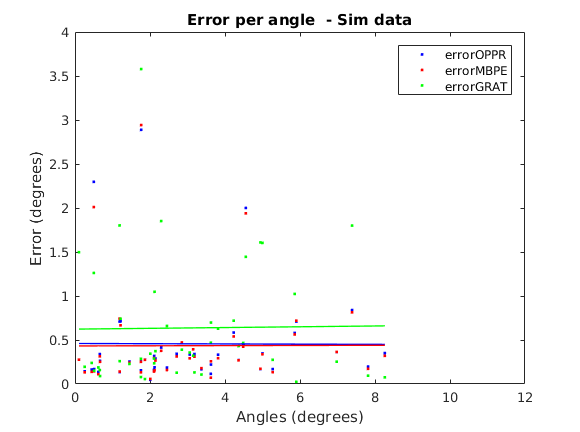
\includegraphics[width=\textwidth]{images/sim/10anglez.png}
	\captionof{figure}{Error per saccade amplitude (in degrees) under simulation on the torsional axis.}
	\label{cha5:sec1:10anglez}
\end{minipage}
\begin{table}
	\centering
	\begin{tabular}{| l | l | l | l |}
		\hline
		Method & X Mean & Y Mean & Z Mean \\
		\hline
		OPPR &  0.33 \degree & 0.54 \degree & 0.46 \degree \\
		\hline
		MBPE &  0.31 \degree & 0.52 \degree & 0.44 \degree\\
		\hline
		GRAT &  0.77 \degree & 1.05 \degree & 0.64 \degree\\ 
		\hline
	\end{tabular}
	\captionof{table}{Mean error (in degrees) per method and per axis.}
	\label{cha5:sec1:10angleaxist}
\end{table}		


\begin{minipage}{0.5\textwidth}
	\centering
	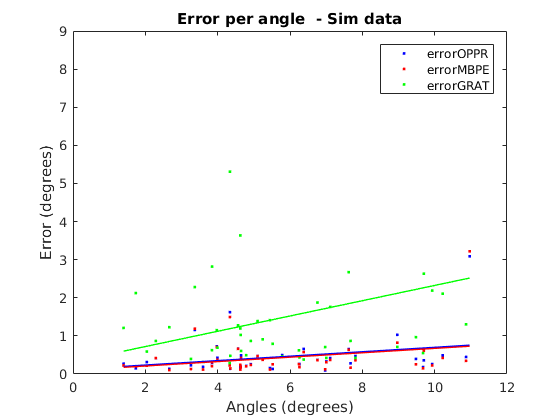
\includegraphics[width=\textwidth]{images/sim/10angle.png}
	\captionof{figure}{Error per saccade amplitude (in degrees) under simulation.}
	\label{cha5:sec1:10angle}
\end{minipage}
\begin{minipage}{0.5\textwidth}
	\centering
	\begin{tabular}{| l | l | l |}
			\hline
			Method & Mean & Standard Deviation \\
			\hline
			OPPR &  0.45 \degree & 0.49 \degree \\
			\hline
			MBPE &  0.42 \degree & 0.50 \degree \\
			\hline
			GRAT &  1.47 \degree & 1.76 \degree \\ 
			\hline
	\end{tabular}
	\captionof{table}{Mean error and standard deviation (in degrees) of the experince on the left per each method tested}
	\label{cha5:sec1:10anglet}
\end{minipage}\\

Robust estimation detected a $ 15.55 \%$ of bad matches.

\subsubsection{Experiment 2 - Saccade amplitudes generated with $\sigma^2 = 15 \degree $}
\begin{minipage}{0.5\textwidth}
	\centering
	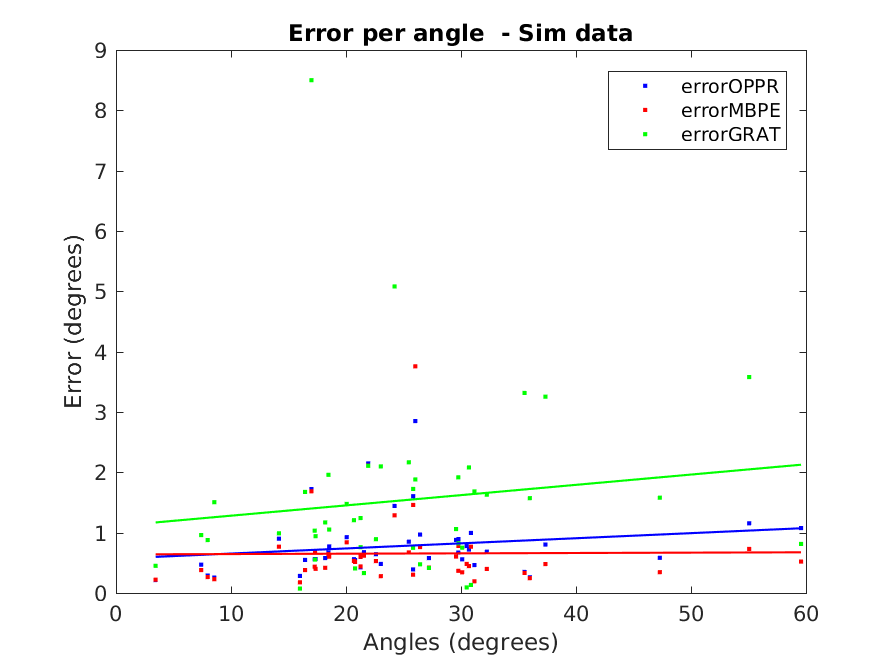
\includegraphics[width=\textwidth]{images/sim/45angle.png}
	\captionof{figure}{Error per saccade amplitude (in degrees) under simulation.}
	\label{cha5:sec1:45angle}
\end{minipage}
\begin{minipage}{0.5\textwidth}
	\centering
	\begin{tabular}{| l | l | l |}
		\hline
		Method & Mean & Standard Deviation \\
		\hline
		OPPR &  0.77 \degree & 0.49 \degree \\
		\hline
		MBPE &  0.65 \degree & 0.60 \degree \\
		\hline
		GRAT &  1.53 \degree & 1.43 \degree \\ 
		\hline
	\end{tabular}
	\captionof{table}{Mean error and standard deviation (in degrees) of the experince on the left per each method tested}
	\label{cha5:sec1:45anglet}
\end{minipage}\\

Robust estimation detected a $ 22.55 \%$ of bad matches.

\subsubsection{Overview}



\subsection{Variable noise}
\subsubsection{Simulation Parameters}
\begin{itemize}
	\item Maximum Matches : $30$
	\item Good Matches : $50 \%$ of the maximum matches
	\item False Matches : $10 \%$ of maximum matches
	\item Noise $\sigma^2$ : $0-100 \ px$ incrementing $10 \ px$ per iteration
	\item Number of saccades: $45$
	\item Zmin : $0.05 m$
	\item Zmáx : $5 m$
	\item Saccade amplitude $\sigma^2 : 4 \degree $
\end{itemize}
\begin{figure}[ht]
	\centering
	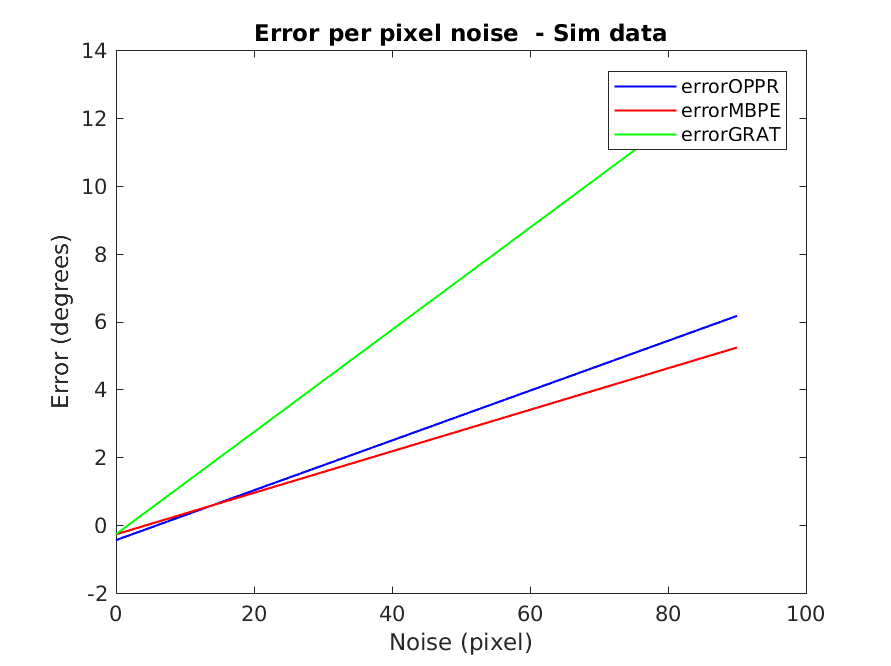
\includegraphics[width=0.5\textwidth]{images/sim/noise.png}
	\captionof{figure}{Error (in degrees) per Gaussian noise in the simulated image (in pixels).}
	\label{cha5:sec1:noise}
\end{figure}
\subsubsection{Overview}

\subsection{Variable baseline}
\subsection{Variable depth}

\subsection{Effect of RANSAC}

\section{Real System}
\subsection{Rotation estimation error}
\subsubsection{Data collection}
\subsubsection{System Parameters}
\begin{itemize}
	\item Maximum Matches : $30$
	\item Good Matches : $50 \%$ of the maximum matches
	\item Zmin : $0.05 m$
	\item Zmáx : $5 m$
	\item Saccade amplitude : random
\end{itemize}
\subsubsection{Experiment 1}
45 saccades were done.\\
\begin{minipage}{0.5\textwidth}
\centering
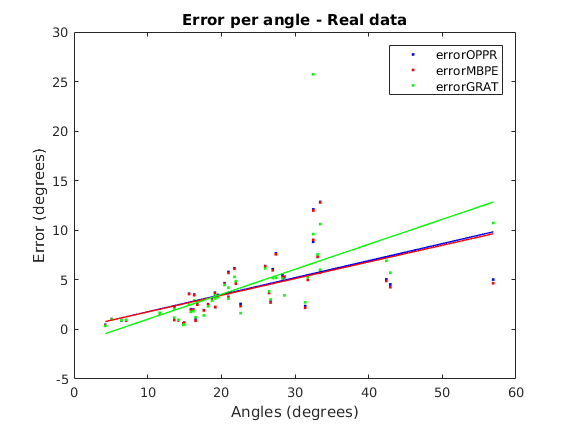
\includegraphics[width=\textwidth]{images/sim/r1angle.png}
\captionof{figure}{Error per saccade amplitude (in degrees) under the real system.}
\label{cha5:sec1:r1angle}
\end{minipage}
\begin{minipage}{0.5\textwidth}
\centering
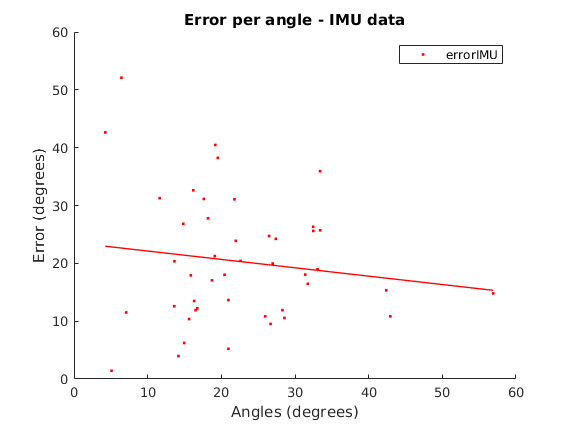
\includegraphics[width=\textwidth]{images/sim/r1angleimu.png}
\captionof{figure}{Error per saccade amplitude (in degrees) under simulation.}
\label{cha5:sec1:r1angleimu}
\end{minipage}\\

\begin{table}
	\centering
\begin{tabular}{| l | l | l |}
	\hline
	Method & Mean & Standard Deviation \\
	\hline
	OPPR &  3.90 \degree & 2.75 \degree \\
	\hline
	MBPE &  3.83 \degree & 2.75 \degree \\
	\hline
	GRAT &  4.13 \degree & 4.09 \degree \\ 
	\hline
	IMU &  20.34 \degree & 10.85 \degree \\ 
	\hline
\end{tabular}
\captionof{table}{Mean error and standard deviation (in degrees) of the experince on the left per each method tested}
\label{cha5:sec1:r1anglet}
\end{table}

Robust estimation detected a $ 94.96 \%$ of bad matches.

\subsubsection{Overview}

\subsubsection{Experiment 2}
32 saccades were done.\\
\begin{minipage}{0.5\textwidth}
	\centering
	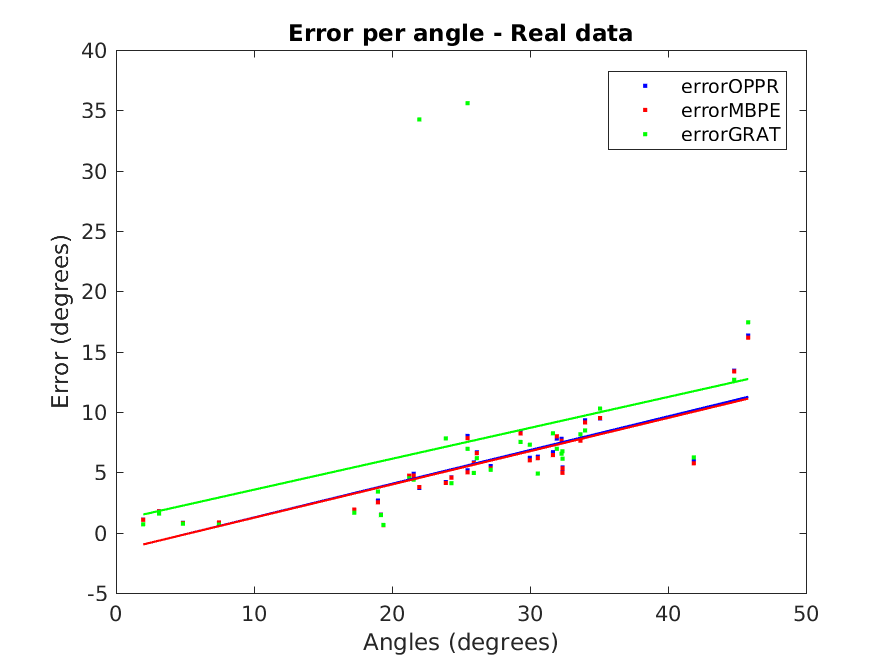
\includegraphics[width=\textwidth]{images/sim/r2angle.png}
	\captionof{figure}{Error per saccade amplitude (in degrees) under simulation.}
	\label{cha5:sec1:r2angle}
\end{minipage}
\begin{minipage}{0.5\textwidth}
	\centering
	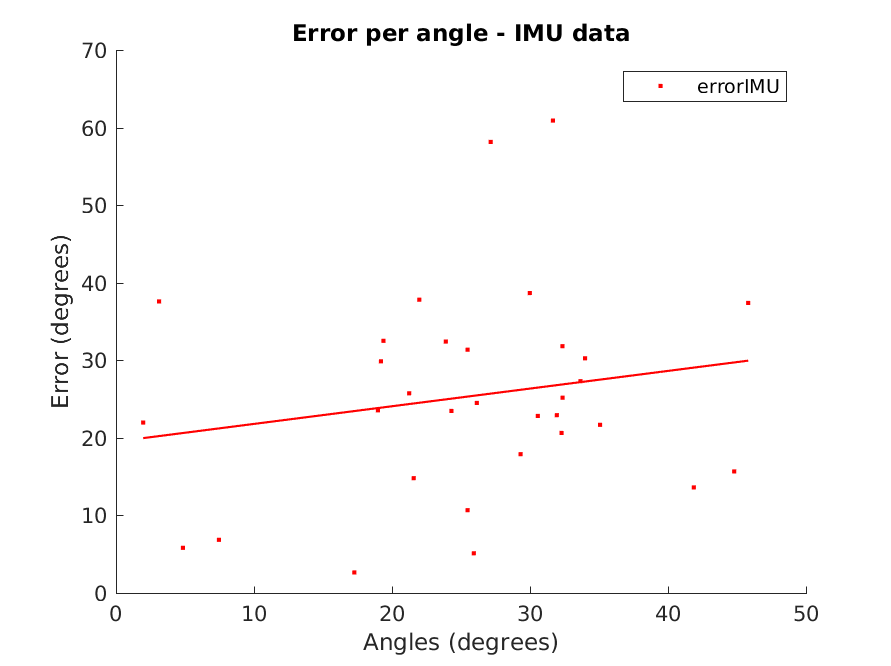
\includegraphics[width=\textwidth]{images/sim/r2angleimu.png}
	\captionof{figure}{Error per saccade amplitude (in degrees) under simulation.}
	\label{cha5:sec1:r2angleimu}
\end{minipage}\\

\begin{table}
	\centering
	\begin{tabular}{| l | l | l |}
		\hline
		Method & Mean & Standard Deviation \\
		\hline
		OPPR &  5.63 \degree & 3.43 \degree \\
		\hline
		MBPE &  5.55 \degree & 3.40 \degree \\
		\hline
		GRAT &  7.57 \degree & 7.79 \degree \\ 
		\hline
		IMU &  25.36 \degree & 13.13 \degree \\ 
		\hline
	\end{tabular}
	\captionof{table}{Mean error and standard deviation (in degrees) of the experince on the left per each method tested}
	\label{cha5:sec1:r2anglet}
\end{table}

Robust estimation detected a $ 93.68 \%$ of bad matches.


\subsubsection{Overview}



\subsection{Effect of RANSAC}


\subsection{Computational speed}